\chapter{Fitting Peak Positions}
\label{Chap:peakpositions}

Fitting the positions for diffraction peaks is an absolutely necessary step in the process for obtaining an accurate structural model. There are only a few challenges to do this. The first is starting with lattice parameters that are close enough to correct to provide significant peak overlap before refining lattice constants. 
The second is that one must select the appropriate corrections for the experimental artifacts that can offset peak positions to be refined, but this is done only after a good fit is obtained. 
Note that it is not sufficient if only one zone of reflections overlaps. For example, the 0\textit{k}0 reflections only provide information about the length of the \textit{b} axis, which is not sufficient to define the axes lengths even in a tetragonal cell. If \textit{n} is the number of unique axes in a cell, for example 2 for hexagonal and 4 for monoclinic, one needs at least \textit{n} and preferably \textit{2n} reflections where \textit{h}, \textit{k} and \textit{l} each have two different values, such as (001), (101) and (030) are all different to be overlapped between the observed and computed patterns, so that that every lattice constant length is defined. High order reflections may not align as well as low Q reflections. It is usually fine to start refining lattice constants even if the high Q reflections are not overlapped, as long as for each axis there are some low order reflections are at least partly aligned. 

In GSAS-II there are several ways to visually confirm that lattice parameters generate peak positions that do a reasonable job of overlapping with the observed peaks in the pattern. For all three, I will assume that you have both a histogram and a phase already imported into a GSAS-I project. 

\section{Ensuring partial peak alignment}

The first approach is to compare the observed and computed patterns and verify that enough reflections are indeed overlapped. This requires that the Calculate/Refine menu command has been run at least once, as this is needed to obtain a computed pattern. It also requires that you have a reasonable value for the histogram scale factor, as it is not possible to view both patterns on the same scale when the histogram scale factor is too far off from correct. 

\subsubsection{Manual scale factor setting}\label{manualscale}
Alas, when peak positions are off from the correct positions, one cannot obtain a good fit for the scale factor for a histogram by refining it, because when a calculated peak is not at the location of the observed peak, the optimal scaling factor that minimizes the differences between the observed and calculated patterns will reduce the peak heights considerably. When faced with this situation, I will sometimes manually force the scale factor to a value that is in the right range so that I can see the computed pattern on the same scale as the observed pattern. To do this, is important to understand that when the number of least-squares cycles is set to zero and a refinement is run, the powder diffraction pattern(s) are computed, but no changes are made to any of the parameters that have been selected to be refined. Thus, selecting the Controls data tree item and setting "Max cycles" to 0 followed by use of the Calculate/Refine menu item will cause the current parameter values to be used to compute the calculated pattern without attempting to optimize any of the parameters that have been set to be refined. With a few repetitions of this, while changing the "Histogram scale factor" value in the Histogram's Sample Parameters data tree item, initially by an order of magnitude or more, allows the computed powder diffraction pattern to be seen on approximately the same scale as the observed pattern. 

\subsection{Use of tick marks}
The second approach also requires that the Calculate/Refine menu command have been run at least once, but is not dependent on the scale factor. After a pattern is computed, the reflection tick mark positions can be displayed visible if either the main "PWDR" or "Reflection list" tree entries are selected. The tick marks can be compared to the peak positions in the observed pattern. Pressing the "f" key to toggle between the three modes used to display the reflection positions. I find that the "full-length" tick marks are best to make clear if computed reflection positions provide overlap with the computed positions. When the Reflections List tree item is selected and the mouse is allowed to "rest" on a short tick mark, the \textit{hkl} value for the reflection is displayed temporarily (aka a "tooltip"). This is not done with "full-length" tick marks or from the "PWDR" tree item.  Reflections can be labeled with their \textit{hkl} indices by right-clicking on the tick mark. Again this is only possible with short tick marks, not the full-length ones, and can be done with either the PDWR or the Reflection Lists tree item. 

\subsection{Interactive cell manipulation}
The third option uses the histogram's Unit Cells List data tree item. The second section of that window, labeled "Unit Cell \& Symmetry Settings for Reflection Display" has inputs for symmetry and lattice constants. The "Cell Index/Refine"/"Load Phase" will load the values into these inputs. The "show HKL from cell" button will cause vertical lines to be placed at the positions where reflections are computed. Note the tiny up and down arrow to the right of each unit cell constant. This will change that lattice constant by a small fraction and the vertical lines will have their positions updated. Change the "Cell step" value to increase or decrease the amount of change associated with each press of the arrow button. The nice thing about using this part of the program is that if the lattice constants do need to be adjusted prior to their use in a refinement, it can be done quickly here. When the mouse is placed over a vertical line, the reflection indices will be displayed will also be displayed as a tooltip. Note that if you find better lattice constants with this process, you will need to make the changes yourself to the values entered for the phase. 

\section{Sample displacement parameters}\label{ref:SampleDisplacement}
After a good fit is obtained for the unit cell constants, noted by the tick marks now well aligned to the reflection positions, this should be optimized by refinement of an appropriate sample parameter, but do not do this until the reflection positions are well fit. 
\begin{itemize}
    \item For Bragg-Brentano Diffraction: for all types of samples refine the "Sample displacement" value. Note that the units for this correction are in microns ($1 \times 10^{-6} m$). For samples composed of low-Z materials, you should also refine the sample transparency correction (see section \ref{sample transparency}.)

\item For Debye-Scherrer X-ray Diffraction: one should always refine the "Sample X displ. perp. to beam" (sample displacement perpendicular to beam) value. 

\item For Debye-Scherrer Neutron Diffraction: one should always refine the "Sample X displ. perp. to beam" (sample displacement perpendicular to beam) value. If data are collected well above $120^\circ\ 2\theta$ one can also refine the "Sample Y displ. || to beam" (sample displacement parallel to beam) in addition. In theory, this second parameter could be refined with x-rays as well, but it is so rare to have much data observed at very high angles.

\item For TOF diffraction, the sample placement can affect the effective distance of the sample from the source. Refining the DIFC Instrument parameter can adjust for this, but it is usually not necessary.  
\end{itemize}

Note that with older software, one would vary the $2\theta$ or TOF zero correction. This correction is available in GSAS-II but does not properly apply the correct shift for a misplaced sample and should not normally be used. 

\section{Visual inspection tips}
After fitting the lattice parameters, view the difference between the observed and computed pattern. When peaks are well aligned, any remaining unfit intensity will appear largely symmetrical. When peaks are not well aligned, the difference has what I call a "derivative" shape, looking something like the first derivative of the peak. Compare Figs. \ref{fig:goodfit} and \ref{fig:notsogoodfit}. In \ref{fig:goodfit} the difference curve shows that there is a bit of intensity in each peak that is not accounted for by the model, but the extra intensity is symmetrical around the peak position, while in \ref{fig:notsogoodfit} note how the difference curve starts positive below the peak but then goes negative above the peak. This latter curve is characteristic of what the difference curve will look like where the calculated peak is not aligned with the data.  Small deviations in peak positions may remain, and require inclusion of the  appropriate instrumental parameter to be fit, and there certainly may be significant differences between the observed and calculated peak intensities, but the the peaks largely should be aligned. If not, the question to consider will be, did not model not converge because it was not started close enough to the correct values for the lattice parameter or is this not the correct cell? In one structure that kept me stumped for weeks, the lower angle data for a fit of Faujasite gave me an excellent fit, but above some value, the peaks were poorly aligned. It turns out that the problem was that the symmetry of the material had dropped and the cell was now orthorhombic. I had not considered that because everyone who works with zeolites knows that Faujasite is cubic. 

\begin{figure}
    \centering
    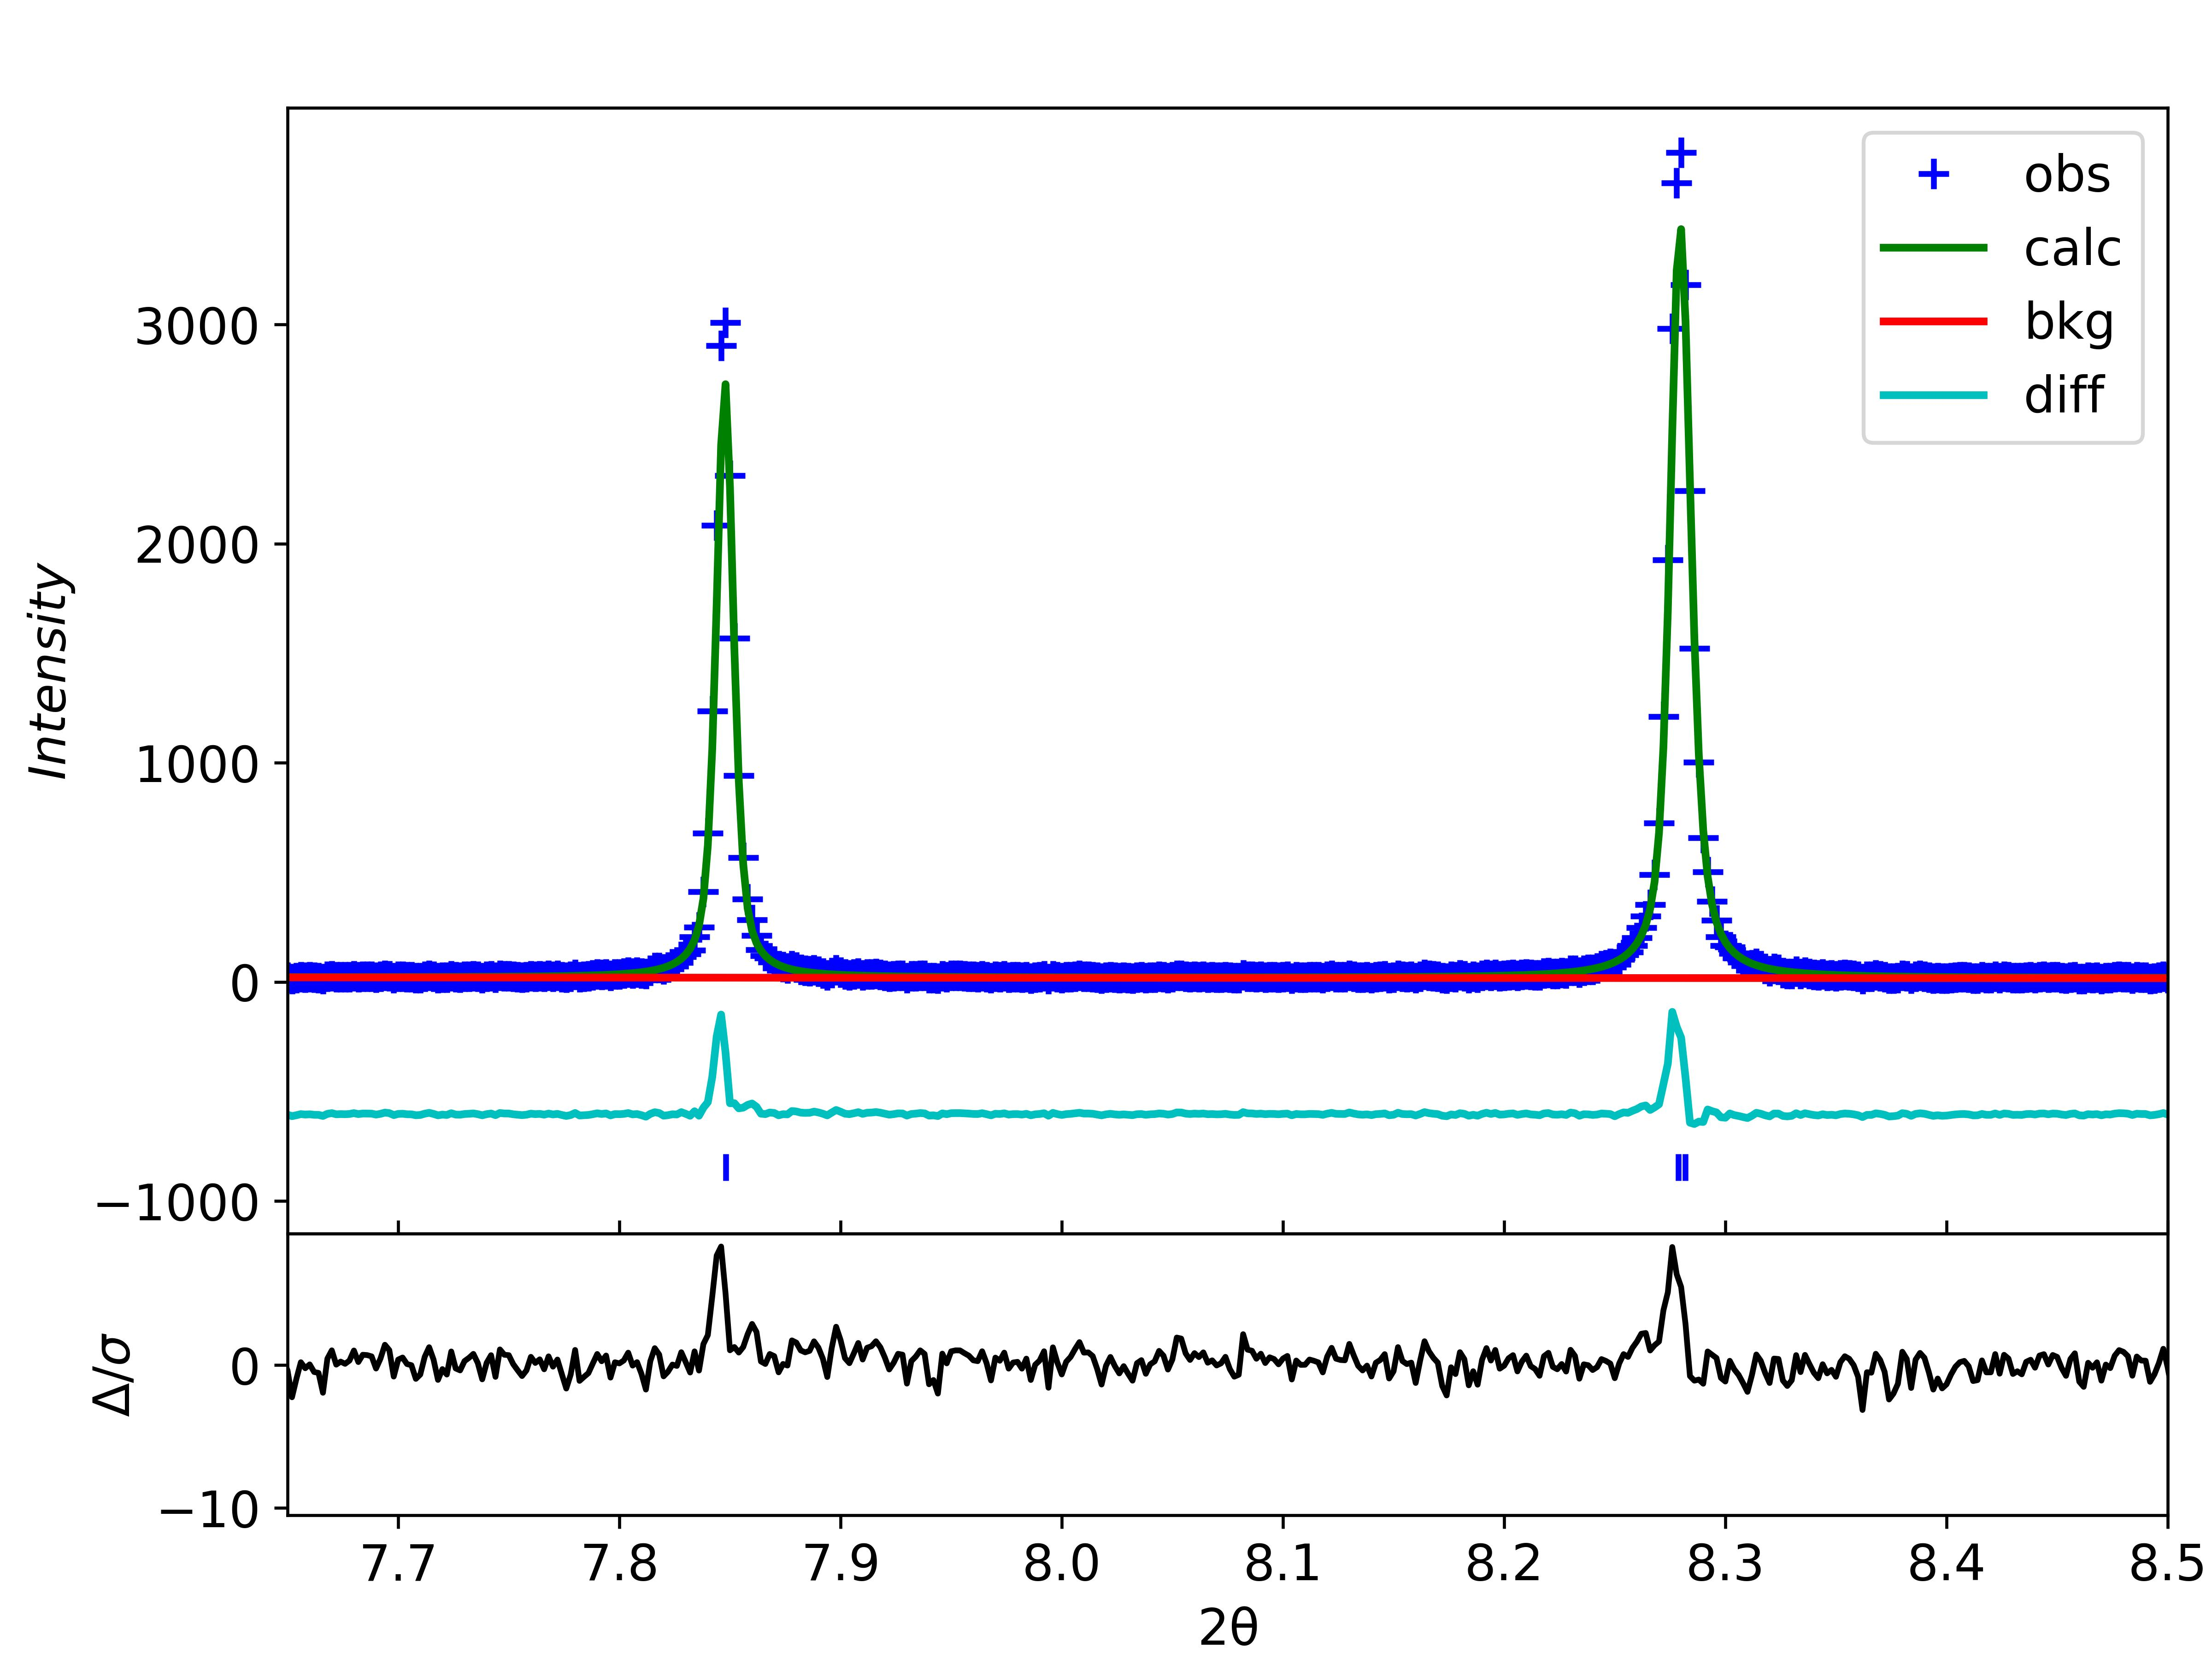
\includegraphics[width=0.5\linewidth]{figures/erice1.jpg}
    \caption{Example fit where calculated peaks are aligned with data}
    \label{fig:goodfit}
\end{figure}
\begin{figure}
        \centering
        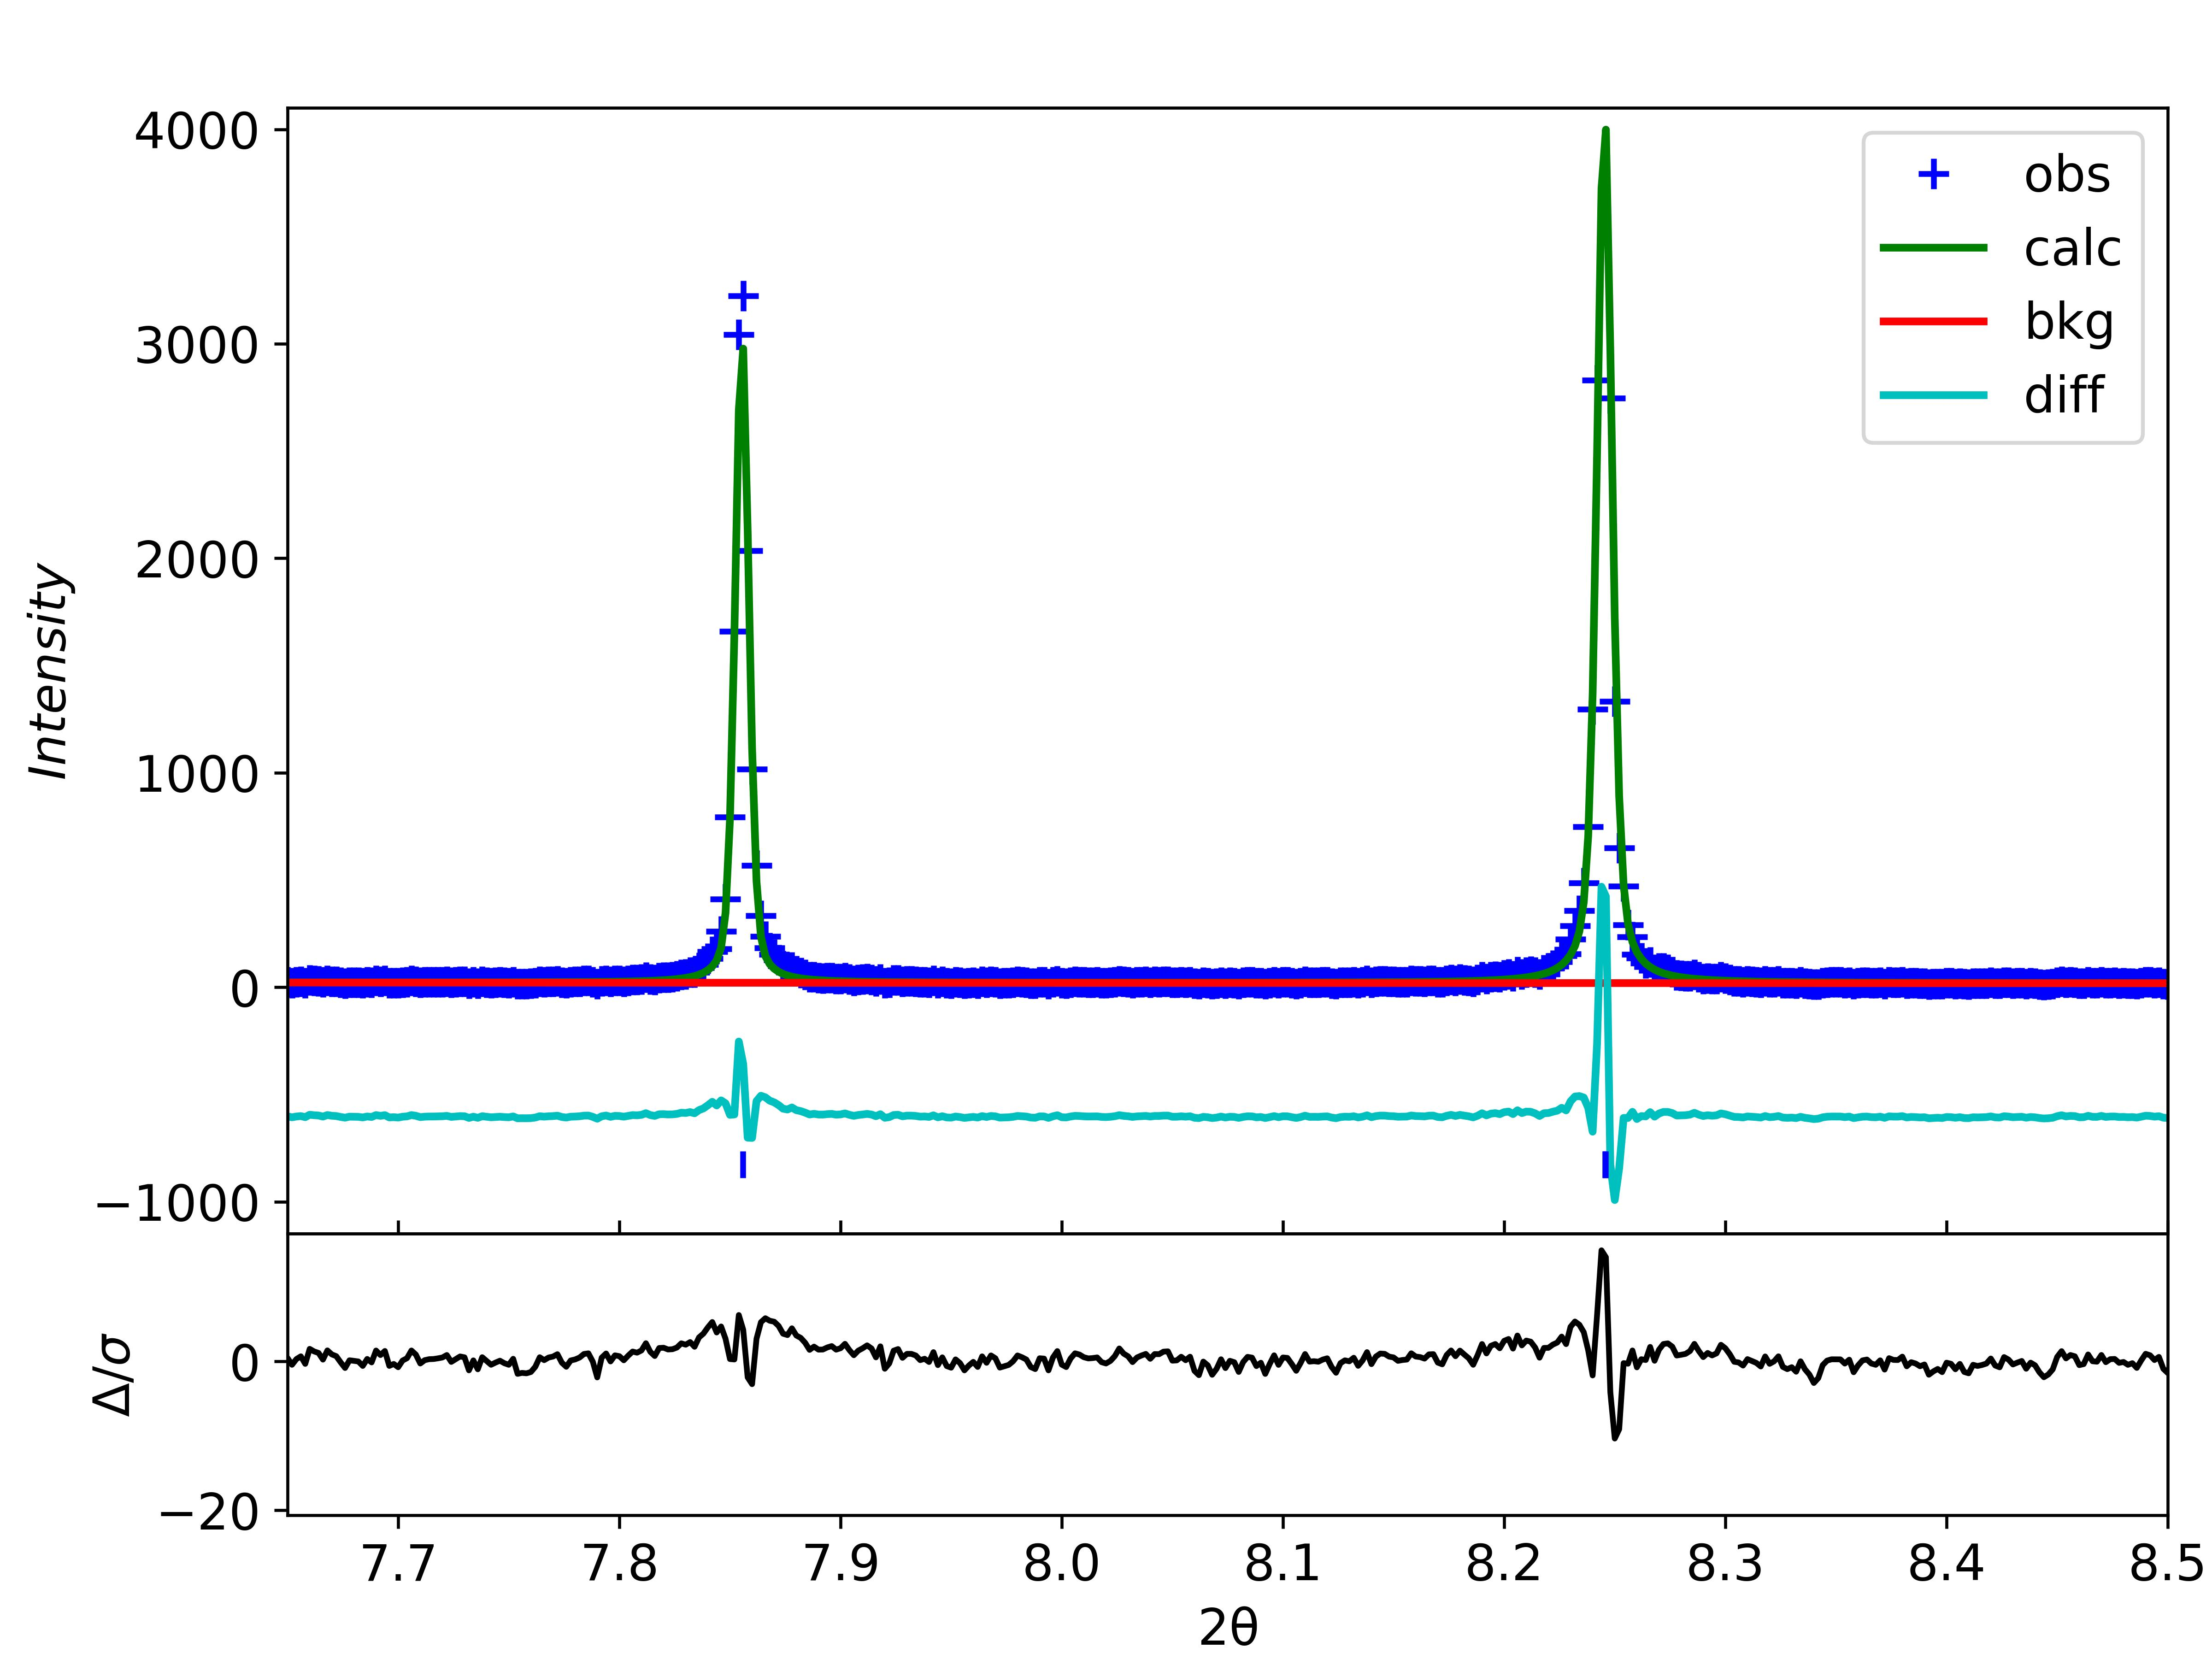
\includegraphics[width=0.5\linewidth]{figures/erice2.jpg}
    \caption{Example fit where calculated peaks are poorly aligned with data}        \label{fig:notsogoodfit}
\end{figure}
Assuming that the fit of the lattice parameters is good, add the appropriate sample parameters into the fit and again view the difference between the observed and computed pattern. There should be no indications that any peaks are misaligned.

\section{Lattice Parameter Precision and Accuracy}

Full pattern fitting is one of the most accurate and precise methods available for determination of lattice constants, at least amongst techniques that are routinely available. Lattice constant determination is one of the few areas where powder diffraction routinely exceeds single-crystal measurements. Between powder techniques, high resolution synchrotron measurements have probably the greatest precision, though neutron measurements, with their improved sensitivity for high Q scattering, may sometimes be even better, but it should be noted that when it comes to accuracy, neither has the advantage that laboratory instruments have in that the characteristic x-ray wavelengths have been standardized to much better accuracy than can be achieved for calibration of a neutron or synchrotron beamline. While I do not normally recommend use of an internal standard in powder diffraction, if obtaining the ultimate in precision and accuracy is desired, use of a high-resolution instrument at either a synchrotron or neutron source with a primary standard integrated into the sample would likely provide the best compromise between precision and accuracy. 

It should be noted that if an accurate structural model is not available for the material where lattice parameters are to be determined, a traditional Rietveld fit may not perform as well as desired, as the intensity mismatch could perturb the lattice fit. Use of a Pawley or Le Bail fit (see section \ref{ref:LeBail}), will avoid that problem. 